% Options for packages loaded elsewhere
% Options for packages loaded elsewhere
\PassOptionsToPackage{unicode}{hyperref}
\PassOptionsToPackage{hyphens}{url}
\PassOptionsToPackage{dvipsnames,svgnames,x11names}{xcolor}
%
\documentclass[
  letterpaper,
  DIV=11,
  numbers=noendperiod]{scrreprt}
\usepackage{xcolor}
\usepackage{amsmath,amssymb}
\setcounter{secnumdepth}{5}
\usepackage{iftex}
\ifPDFTeX
  \usepackage[T1]{fontenc}
  \usepackage[utf8]{inputenc}
  \usepackage{textcomp} % provide euro and other symbols
\else % if luatex or xetex
  \usepackage{unicode-math} % this also loads fontspec
  \defaultfontfeatures{Scale=MatchLowercase}
  \defaultfontfeatures[\rmfamily]{Ligatures=TeX,Scale=1}
\fi
\usepackage{lmodern}
\ifPDFTeX\else
  % xetex/luatex font selection
\fi
% Use upquote if available, for straight quotes in verbatim environments
\IfFileExists{upquote.sty}{\usepackage{upquote}}{}
\IfFileExists{microtype.sty}{% use microtype if available
  \usepackage[]{microtype}
  \UseMicrotypeSet[protrusion]{basicmath} % disable protrusion for tt fonts
}{}
\makeatletter
\@ifundefined{KOMAClassName}{% if non-KOMA class
  \IfFileExists{parskip.sty}{%
    \usepackage{parskip}
  }{% else
    \setlength{\parindent}{0pt}
    \setlength{\parskip}{6pt plus 2pt minus 1pt}}
}{% if KOMA class
  \KOMAoptions{parskip=half}}
\makeatother
% Make \paragraph and \subparagraph free-standing
\makeatletter
\ifx\paragraph\undefined\else
  \let\oldparagraph\paragraph
  \renewcommand{\paragraph}{
    \@ifstar
      \xxxParagraphStar
      \xxxParagraphNoStar
  }
  \newcommand{\xxxParagraphStar}[1]{\oldparagraph*{#1}\mbox{}}
  \newcommand{\xxxParagraphNoStar}[1]{\oldparagraph{#1}\mbox{}}
\fi
\ifx\subparagraph\undefined\else
  \let\oldsubparagraph\subparagraph
  \renewcommand{\subparagraph}{
    \@ifstar
      \xxxSubParagraphStar
      \xxxSubParagraphNoStar
  }
  \newcommand{\xxxSubParagraphStar}[1]{\oldsubparagraph*{#1}\mbox{}}
  \newcommand{\xxxSubParagraphNoStar}[1]{\oldsubparagraph{#1}\mbox{}}
\fi
\makeatother


\usepackage{longtable,booktabs,array}
\usepackage{calc} % for calculating minipage widths
% Correct order of tables after \paragraph or \subparagraph
\usepackage{etoolbox}
\makeatletter
\patchcmd\longtable{\par}{\if@noskipsec\mbox{}\fi\par}{}{}
\makeatother
% Allow footnotes in longtable head/foot
\IfFileExists{footnotehyper.sty}{\usepackage{footnotehyper}}{\usepackage{footnote}}
\makesavenoteenv{longtable}
\usepackage{graphicx}
\makeatletter
\newsavebox\pandoc@box
\newcommand*\pandocbounded[1]{% scales image to fit in text height/width
  \sbox\pandoc@box{#1}%
  \Gscale@div\@tempa{\textheight}{\dimexpr\ht\pandoc@box+\dp\pandoc@box\relax}%
  \Gscale@div\@tempb{\linewidth}{\wd\pandoc@box}%
  \ifdim\@tempb\p@<\@tempa\p@\let\@tempa\@tempb\fi% select the smaller of both
  \ifdim\@tempa\p@<\p@\scalebox{\@tempa}{\usebox\pandoc@box}%
  \else\usebox{\pandoc@box}%
  \fi%
}
% Set default figure placement to htbp
\def\fps@figure{htbp}
\makeatother





\setlength{\emergencystretch}{3em} % prevent overfull lines

\providecommand{\tightlist}{%
  \setlength{\itemsep}{0pt}\setlength{\parskip}{0pt}}



 


\usepackage[makeroom]{cancel}
\def\eb{\boldsymbol{e}}
\def\fb{\boldsymbol{f}}
\def\hb{\boldsymbol{h}}
\def\xb{\boldsymbol{x}}
\def\Rb{\boldsymbol{R}}
\def\Real{\mathbb{R}}
\def\bfzero{\boldsymbol{0}}
\newcommand{\ddy}[2]{\frac{\partial{#1}}{\partial{#2}}}
\DeclareOldFontCommand{\bf}{\normalfont\bfseries}{\mathbf}
\DeclareOldFontCommand{\rm}{\normalfont\rmseries}{\mathrm}
\KOMAoption{captions}{tableheading}
\makeatletter
\@ifpackageloaded{tcolorbox}{}{\usepackage[skins,breakable]{tcolorbox}}
\@ifpackageloaded{fontawesome5}{}{\usepackage{fontawesome5}}
\definecolor{quarto-callout-color}{HTML}{909090}
\definecolor{quarto-callout-note-color}{HTML}{0758E5}
\definecolor{quarto-callout-important-color}{HTML}{CC1914}
\definecolor{quarto-callout-warning-color}{HTML}{EB9113}
\definecolor{quarto-callout-tip-color}{HTML}{00A047}
\definecolor{quarto-callout-caution-color}{HTML}{FC5300}
\definecolor{quarto-callout-color-frame}{HTML}{acacac}
\definecolor{quarto-callout-note-color-frame}{HTML}{4582ec}
\definecolor{quarto-callout-important-color-frame}{HTML}{d9534f}
\definecolor{quarto-callout-warning-color-frame}{HTML}{f0ad4e}
\definecolor{quarto-callout-tip-color-frame}{HTML}{02b875}
\definecolor{quarto-callout-caution-color-frame}{HTML}{fd7e14}
\makeatother
\makeatletter
\@ifpackageloaded{bookmark}{}{\usepackage{bookmark}}
\makeatother
\makeatletter
\@ifpackageloaded{caption}{}{\usepackage{caption}}
\AtBeginDocument{%
\ifdefined\contentsname
  \renewcommand*\contentsname{Table of contents}
\else
  \newcommand\contentsname{Table of contents}
\fi
\ifdefined\listfigurename
  \renewcommand*\listfigurename{List of Figures}
\else
  \newcommand\listfigurename{List of Figures}
\fi
\ifdefined\listtablename
  \renewcommand*\listtablename{List of Tables}
\else
  \newcommand\listtablename{List of Tables}
\fi
\ifdefined\figurename
  \renewcommand*\figurename{Figure}
\else
  \newcommand\figurename{Figure}
\fi
\ifdefined\tablename
  \renewcommand*\tablename{Table}
\else
  \newcommand\tablename{Table}
\fi
}
\@ifpackageloaded{float}{}{\usepackage{float}}
\floatstyle{ruled}
\@ifundefined{c@chapter}{\newfloat{codelisting}{h}{lop}}{\newfloat{codelisting}{h}{lop}[chapter]}
\floatname{codelisting}{Listing}
\newcommand*\listoflistings{\listof{codelisting}{List of Listings}}
\makeatother
\makeatletter
\makeatother
\makeatletter
\@ifpackageloaded{caption}{}{\usepackage{caption}}
\@ifpackageloaded{subcaption}{}{\usepackage{subcaption}}
\makeatother
\makeatletter
\@ifpackageloaded{tcolorbox}{}{\usepackage[many]{tcolorbox}}
\makeatother
%%%% ---foldboxy preamble ----- %%%%%

\definecolor{fbx-default-color1}{HTML}{c7c7d0}
\definecolor{fbx-default-color2}{HTML}{a3a3aa}

\definecolor{fbox-color1}{HTML}{c7c7d0}
\definecolor{fbox-color2}{HTML}{a3a3aa}

% arguments: #1 typelabelnummer: #2 titel: #3
\newenvironment{fbx}[3]{\begin{tcolorbox}[enhanced, breakable,%
attach boxed title to top*={xshift=1.4pt},
boxed title style={boxrule=0.0mm, fuzzy shadow={1pt}{-1pt}{0mm}{0.1mm}{gray}, arc=.3em, rounded corners=east, sharp corners=west}, colframe=#1-color2, colbacktitle=#1-color1, colback = white, coltitle=black,  titlerule=0mm, toprule=0pt, bottomrule=.7pt, leftrule=.3em, rightrule=0pt, outer arc=.3em,  arc=0pt,	 sharp corners = east, left=.5em, bottomtitle=1mm, toptitle=1mm,title=\textbf{#2}\hspace{0.5em}{#3}]}
{\end{tcolorbox}}

% boxed environment with right border
\newenvironment{fbxSimple}[3]{\begin{tcolorbox}[enhanced, breakable,%
attach boxed title to top*={xshift=1.4pt},
boxed title style={boxrule=0.0mm, fuzzy shadow={1pt}{-1pt}{0mm}{0.1mm}{gray}, arc=.3em, rounded corners=east, sharp corners=west}, colframe=#1-color2, colbacktitle=#1-color1, colback = white, coltitle=black,  titlerule=0mm, toprule=0pt, bottomrule=.7pt, leftrule=.3em, rightrule=.7pt, outer arc=.3em,  	left=.5em, right=.5em, bottomtitle=1mm, toptitle=1mm,title=\textbf{#2}\hspace{0.5em}{#3}]}
{\end{tcolorbox}}

%%%% --- end foldboxy preamble ----- %%%%%
%%==== colors from yaml ===%
\definecolor{doit-color1}{HTML}{e7efea}
\definecolor{doit-color2}{HTML}{53b57b}
\definecolor{theorem-color1}{HTML}{fcebee}
\definecolor{theorem-color2}{HTML}{ea3342}
\definecolor{eg-color1}{HTML}{E7D6EA}
\definecolor{eg-color2}{HTML}{68246D}
%=============%
\usepackage{bookmark}
\IfFileExists{xurl.sty}{\usepackage{xurl}}{} % add URL line breaks if available
\urlstyle{same}
\hypersetup{
  pdftitle={Computational Mathematics II (MATH2731)},
  pdfauthor={Dr Andrew Krause \& Dr Denis Patterson, Durham University},
  colorlinks=true,
  linkcolor={blue},
  filecolor={Maroon},
  citecolor={Blue},
  urlcolor={Blue},
  pdfcreator={LaTeX via pandoc}}


\title{Computational Mathematics II (MATH2731)}
\author{Dr Andrew Krause \& Dr Denis Patterson, Durham University}
\date{2025-06-01}
\begin{document}
\maketitle

\renewcommand*\contentsname{Table of contents}
{
\hypersetup{linkcolor=}
\setcounter{tocdepth}{2}
\tableofcontents
}

\bookmarksetup{startatroot}

\chapter*{Introduction}\label{introduction}
\addcontentsline{toc}{chapter}{Introduction}

\markboth{Introduction}{Introduction}

\textbf{Welcome to Computational Mathematics II!}

This course aims to help you build skills and knowledge in using modern
computational methods to do and apply mathematics. It will involve a
blend of hands-on computing work and mathematical theory---this theory
will include aspects of numerical analysis, computational algebra, and
other topics within scientific computing. These areas consist of
studying the mathematical properties of the computational
representations of mathematical objects (numerical values as well as
symbolic manipulations). The computing skills developed in this module
will be valuable in all subsequent courses in your degree at Durham and
well beyond. We will also introduce you to the use (and abuse) of
various computational tools invaluable for doing mathematics, such as AI
and searchable websites. While we will encourage you throughout to use
all the tools at your disposal, it is \textbf{imperative that you
understand the details and scope of what you are doing!} You will also
develop your communication, presentation, and group-work skills through
the various assessments involved in the course -- more on that below!

This module has \textbf{no final exam}. In fact, there are no exams of
any kind. Instead, the summative assessment and associated final grade
are entirely based on coursework undertaken during the term. This means
that you should expect to spend more time on this course during the term
relative to your other modules. We believe this workload distribution is
a better way to train the skills we are trying to develop, and as a
bonus, you will not need to worry about this course any further once the
term ends!

\begin{center}\rule{0.5\linewidth}{0.5pt}\end{center}

\section*{Content}\label{content}
\addcontentsline{toc}{section}{Content}

\markright{Content}

The module's content is divided into six chapters of roughly equal
length; some will focus slightly more on theory, while others have a
more practical and hands-on nature.

\begin{itemize}
\tightlist
\item
  \textbf{Chapter 1: Introduction to Computational Mathematics}

  \begin{itemize}
  \tightlist
  \item
    Programming basics (including GitHub, and numerical versus symbolic
    computation)
  \item
    LaTeX, Overleaf, and presenting lab reports
  \item
    Finite-precision arithmetic, rounding error, symbolic
    representations
  \end{itemize}
\item
  \textbf{Chapter 2: Continuous Functions}

  \begin{itemize}
  \tightlist
  \item
    Interpolation using polynomials -- fitting curves to data (Lagrange
    polynomials, error estimates, convergence, and Chebyshev nodes)
  \item
    Solving nonlinear equations (bisection, fixed-point iteration,
    Newton's method)
  \end{itemize}
\item
  \textbf{Chapter 3: Linear Algebra}

  \begin{itemize}
  \tightlist
  \item
    Solving linear systems numerically (LU decomposition, Gaussian
    elimination, conditioning) and symbolically
  \item
    Applications: PageRank, computer graphics
  \end{itemize}
\item
  \textbf{Chapter 4: Calculus}

  \begin{itemize}
  \tightlist
  \item
    Numerical differentiation (finite differences)
  \item
    Numerical integration (quadrature rules, Newton-Cotes formulae)
  \end{itemize}
\item
  \textbf{Chapter 5: Ordinary Differential Equations (ODEs)}

  \begin{itemize}
  \tightlist
  \item
    Numerically approximating solutions of ODEs
  \item
    Timestepping: explicit and implicit methods
  \item
    Stability and convergence order
  \end{itemize}
\item
  \textbf{Chapter 6: Selected Further Topics}

  \begin{itemize}
  \tightlist
  \item
    Intro. to random numbers and stochastic processes
  \item
    Intro. to partial differential equations
  \end{itemize}
\end{itemize}

\begin{center}\rule{0.5\linewidth}{0.5pt}\end{center}

\section*{Weekly workflow and summative
assessment}\label{weekly-workflow-and-summative-assessment}
\addcontentsline{toc}{section}{Weekly workflow and summative assessment}

\markright{Weekly workflow and summative assessment}

The final grade for this module is determined as follows:

\begin{itemize}
\tightlist
\item
  \textbf{Weekly lab reports (weeks 1-6)} -- 20\%
\item
  \textbf{Weekly e-assessments (weeks 1-6)} -- 30\%
\item
  \textbf{Project (weeks 7-10)} -- 50\%
\end{itemize}

\subsection*{Lab reports}\label{lab-reports}
\addcontentsline{toc}{subsection}{Lab reports}

Each week for the first six weeks of the course, we will release a short
set of exercises based on the lectures from the previous week. Students
will be expected to submit a brief report (1-2 pages A4, including
figures) with their solutions to the set of exercises -- the report will
consist of written answers and figures/plots. The reports will be
evaluated for correctness and quality of the presentation and
communication (quality of figures, clarity of argumentation, etc.).\\
\textbf{The lab report for a given week will be due at noon on Monday of
the following week} (e.g., week one's lab report is due on Monday of
week two and so on). Solutions and generalised feedback will be provided
to the class on common mistakes and issues arising in each report.
Students can also seek detailed feedback on their submission from the
lecturers during drop-in sessions and office hours. There will be six
lab reports in total, and \textbf{your mark is based on your four
highest-scoring submissions.}

\subsection*{E-assessments}\label{e-assessments}
\addcontentsline{toc}{subsection}{E-assessments}

Each week for the first six weeks of the course, we will release an
e-assessment based on the lectures from the previous week. These
exercises are designed to complement the lab reports by focusing
exclusively on coding skills. The e-assessments will involve submitting
code auto-marked by an online grading tool, and hence give immediate
feedback. As with the lab reports, \textbf{the e-assessment for a given
week will be due at noon on Monday of the following week}. There will be
six e-assessments in total, and \textbf{your mark is based on your four
highest-scoring submissions.}

\subsection*{Project}\label{project}
\addcontentsline{toc}{subsection}{Project}

The single largest component of the assessment for this module is the
project. \textbf{Weeks 7-10 of this course focus exclusively on project
work with lectures ending in Week 6.} We will be releasing more detailed
instructions on the project submission format and assessment criteria
separately, but briefly, the main aspects of the project are as follows:

\begin{itemize}
\tightlist
\item
  There will be approximately eight different project options to choose
  from across different areas of mathematics (e.g., pure, applied,
  probability, mathematical physics, etc.); each project has a distinct
  member of the Maths Department as supervisor.
\item
  Students will submit their preferred project options (ranked choice
  preferences) in Week 4 of the term and be allocated to projects by the
  end of Week 6 (there are maximum subscription numbers for each option
  to ensure equity of supervision).
\item
  Each project consists of two parts: a \textbf{guided component} that
  is completed as part of a small group and an \textbf{extension
  component} that is open-ended and completed as an individual. Group
  allocations will be done by the lecturers.
\item
  Each group will jointly submit a five-page report for the guided
  component of the project, and this is worth 60\% of the project grade.
\item
  Each student will also submit a three-page report and a six-minute
  video presentation on their extension component. This submission is
  worth 40\% of the project grade.
\end{itemize}

In Weeks 7-10 of the term, lectures will be replaced by project workshop
sessions during which students can discuss their project with the
designated supervisor. This will be an opportunity to discuss progress,
ask questions, and seek clarification. Each student only needs to attend
the one project drop-in weekly session relevant to their project.
Computing drop-in sessions will continue as scheduled in the first six
weeks to provide additional support for coding pertinent tasks for the
projects -- there will be two timetabled computing drop-ins per week and
students are encouraged to attend at least one of them.

\begin{center}\rule{0.5\linewidth}{0.5pt}\end{center}

\section*{Lectures, computing drop-ins \& project
workshops}\label{lectures-computing-drop-ins-project-workshops}
\addcontentsline{toc}{section}{Lectures, computing drop-ins \& project
workshops}

\markright{Lectures, computing drop-ins \& project workshops}

Lectures will primarily present, explain, and discuss new material
(especially theory), but will also feature computer demonstrations of
the algorithms and numerical methods. As such, students are encouraged
to bring their laptops to lectures to run the examples themselves.
Students must bring a laptop or device capable of running code to the
computer drop-ins to work on the e-assessments and lab reports.

\begin{longtable}[]{@{}cll@{}}
\toprule\noalign{}
& Activities & Content \\
\midrule\noalign{}
\endhead
\bottomrule\noalign{}
\endlastfoot
\textbf{Week 1} & Introductory lecture, 2 lectures & Chapter 1 \\
\textbf{Week 2} & 3 lectures, 1 computing drop-in & Chapter 2 \\
\textbf{Week 3} & 3 lectures, 1 computing drop-in & Chapter 3 \\
\textbf{Week 4} & 3 lectures, 1 computing drop-in & Chapter 4 \\
\textbf{Week 5} & 3 lectures, 1 computing drop-in & Chapter 5 \\
\textbf{Week 6} & 3 lectures, 1 computing drop-in & Chapter 5/6 \\
\textbf{Week 7} & 0 lectures, 1 project workshop & Project \\
\textbf{Week 8} & 0 lectures, 1 project workshop & Project \\
\textbf{Week 9} & 0 lectures, 1 project workshop & Project \\
\textbf{Week 10} & 0 lectures, 1 project workshop & Project \\
\end{longtable}

\begin{center}\rule{0.5\linewidth}{0.5pt}\end{center}

\section*{Contact details and Reading
Materials}\label{contact-details-and-reading-materials}
\addcontentsline{toc}{section}{Contact details and Reading Materials}

\markright{Contact details and Reading Materials}

If you have questions or need clarification on any of the above, please
speak to us during lectures, drop-in sessions, or office hours.
Alternatively, email one or both of us at
\href{mailto:denis.d.patterson@durham.ac.uk}{\nolinkurl{denis.d.patterson@durham.ac.uk}}
or
\href{mailto:andrew.krause@durham.ac.uk}{\nolinkurl{andrew.krause@durham.ac.uk}}.

The lecture notes are designed to be sufficient and self-contained.
Hence, students do not need to purchase a textbook to complete the
course successfully. References for additional reading will also be
given at the end of each chapter.

The following texts may be useful supplementary references for students
wishing to read further into topics from the course:

\begin{itemize}
\tightlist
\item
  Burden, R. L., \& Faires, J. D. (1997). \emph{Numerical Analysis} (6th
  ed.). Pacific Grove, CA: Brooks/Cole Publishing Company.
\item
  Süli, E., \& Mayers, D. F. (2003). \emph{An Introduction to Numerical
  Analysis}. Cambridge: Cambridge University Press.
\end{itemize}

\section*{Acknowledgements}\label{acknowledgements}
\addcontentsline{toc}{section}{Acknowledgements}

\markright{Acknowledgements}

We are indebted to Prof.~Anthony Yeates (Durham) who numerical analysis
notes formed the basis of several chapters of the coures notes.

\bookmarksetup{startatroot}

\chapter{Floating Point Arithmetic}\label{floating-point-arithmetic}

The goal of this chapter is to explore and begin to answer the following
question:

\begin{quote}
\emph{How do we represent numbers on a computer?}
\end{quote}

Integers can be represented exactly, up to some maximum size.

If 1 bit (binary digit) is used to store the sign \(\pm\), the largest
possible number is \[
1\times 2^{62} +1\times 2^{61} + \ldots + 1\times 2^{1} + 1\times 2^{0} = 2^{63}-1.
\]

\begin{tcolorbox}[enhanced jigsaw, bottomtitle=1mm, title=\textcolor{quarto-callout-note-color}{\faInfo}\hspace{0.5em}{Note}, colback=white, opacityback=0, rightrule=.15mm, bottomrule=.15mm, colbacktitle=quarto-callout-note-color!10!white, colframe=quarto-callout-note-color-frame, arc=.35mm, breakable, coltitle=black, leftrule=.75mm, left=2mm, toptitle=1mm, toprule=.15mm, titlerule=0mm, opacitybacktitle=0.6]

Some modern languages (such as Python) automatically promote large
integers to arbitrary precision (``long''), but most statically-typed
languages (C, Java, Matlab, etc.) do not; an \textbf{overflow} will
occur and the type remains fixed.

\end{tcolorbox}

By contrast, only a subset of real numbers within any given interval can
be represented exactly.

\section{Fixed-point numbers}\label{fixed-point-numbers}

In everyday life, we tend to use a \textbf{fixed point} representation
\[
x = \pm (d_1d_2\cdots d_{k-1}.d_k\cdots d_n)_\beta, \quad \textrm{where} \quad d_1,\ldots,d_n\in\{0,1,\ldots,\beta - 1\}.
\] Here \(\beta\) is the base (e.g.~10 for decimal arithmetic or 2 for
binary).

If we require that \(d_1\neq 0\) unless \(k=2\), then every number has a
unique representation of this form, except for infinite trailing
sequences of digits \(\beta - 1\).

\section{Floating-point numbers}\label{floating-point-numbers}

Computers use a \textbf{floating-point} representation. Only numbers in
a \textbf{floating-point number system} \(F\subset\mathbb{R}\) can be
represented exactly, where \[
F = \big\{ \pm (0.d_1d_2\cdots d_{m})_\beta\beta^e \;| \;  \beta, d_i, e \in \mathbb{Z}, \;0 \leq d_i \leq \beta-1, \;e_{\rm min} \leq e \leq e_{\rm max}\big\}.
\] Here \((0.d_1d_2\cdots d_{m})_\beta\) is called the \textbf{fraction}
(or \textbf{significand} or \textbf{mantissa}), \(\beta\) is the base,
and \(e\) is the \textbf{exponent}. This can represent a much larger
range of numbers than a fixed-point system of the same size, although at
the cost that the numbers are not equally spaced. If \(d_1\neq 0\) then
each number in \(F\) has a unique representation and \(F\) is called
\textbf{normalised}.

\begin{center}
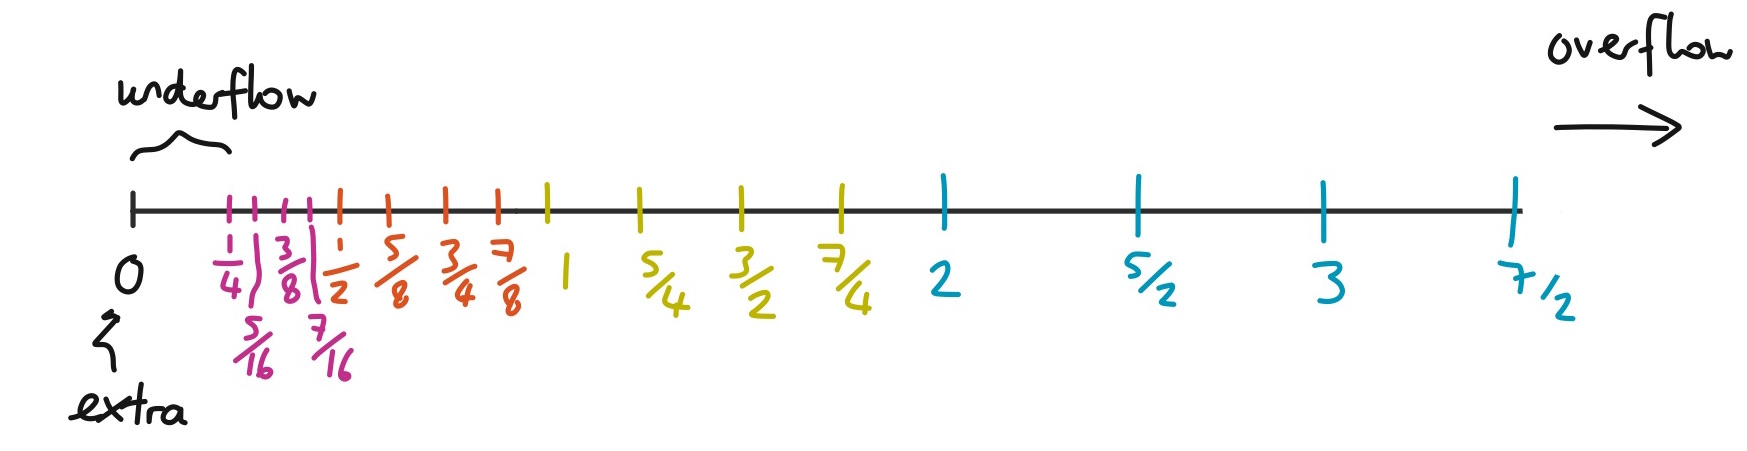
\includegraphics[width=0.7\linewidth,height=\textheight,keepaspectratio]{im/fp1.jpg}
\end{center}

\begin{tcolorbox}[enhanced jigsaw, bottomtitle=1mm, title=\textcolor{quarto-callout-note-color}{\faInfo}\hspace{0.5em}{Note}, colback=white, opacityback=0, rightrule=.15mm, bottomrule=.15mm, colbacktitle=quarto-callout-note-color!10!white, colframe=quarto-callout-note-color-frame, arc=.35mm, breakable, coltitle=black, leftrule=.75mm, left=2mm, toptitle=1mm, toprule=.15mm, titlerule=0mm, opacitybacktitle=0.6]

Notice that the spacing between numbers jumps by a factor \(\beta\) at
each power of \(\beta\). The largest possible number is
\((0.111)_22^2 = (\tfrac12 + \tfrac14 + \tfrac18)(4) = \tfrac72\). The
smallest non-zero number is
\((0.100)_22^{-1}=\tfrac12(\tfrac12) = \tfrac14\).

\end{tcolorbox}

Here \(\beta=2\), and there are 52 bits for the fraction, 11 for the
exponent, and 1 for the sign. The actual format used is \[
\pm (1.d_1\cdots d_{52})_22^{e-1023} = \pm (0.1d_1\cdots d_{52})_22^{e-1022}, \quad e = (e_1e_2\cdots e_{11})_2.
\] When \(\beta=2\), the first digit of a normalized number is always
\(1\), so doesn't need to be stored in memory. The \textbf{exponent
bias} of 1022 means that the actual exponents are in the range \(-1022\)
to \(1025\), since \(e\in[0,2047]\). Actually the exponents \(-1022\)
and \(1025\) are used to store \(\pm 0\) and \(\pm\infty\) respectively.

The smallest non-zero number in this system is
\((0.1)_22^{-1021} \approx 2.225\times 10^{-308}\), and the largest
number is \((0.1\cdots 1)_22^{1024} \approx 1.798\times 10^{308}\).

\begin{tcolorbox}[enhanced jigsaw, bottomtitle=1mm, title=\textcolor{quarto-callout-note-color}{\faInfo}\hspace{0.5em}{Note}, colback=white, opacityback=0, rightrule=.15mm, bottomrule=.15mm, colbacktitle=quarto-callout-note-color!10!white, colframe=quarto-callout-note-color-frame, arc=.35mm, breakable, coltitle=black, leftrule=.75mm, left=2mm, toptitle=1mm, toprule=.15mm, titlerule=0mm, opacitybacktitle=0.6]

IEEE stands for Institute of Electrical and Electronics Engineers.
Matlab uses the IEEE 754 standard for floating point arithmetic. The
automatic 1 is sometimes called the ``hidden bit''. The exponent bias
avoids the need to store the sign of the exponent.

\end{tcolorbox}

Numbers outside the finite set \(F\) cannot be represented exactly. If a
calculation falls below the lower non-zero limit (in absolute value), it
is called \textbf{underflow}, and usually set to 0. If it falls above
the upper limit, it is called \textbf{overflow}, and usually results in
a floating-point exception.

\begin{tcolorbox}[enhanced jigsaw, bottomtitle=1mm, title=\textcolor{quarto-callout-note-color}{\faInfo}\hspace{0.5em}{Note}, colback=white, opacityback=0, rightrule=.15mm, bottomrule=.15mm, colbacktitle=quarto-callout-note-color!10!white, colframe=quarto-callout-note-color-frame, arc=.35mm, breakable, coltitle=black, leftrule=.75mm, left=2mm, toptitle=1mm, toprule=.15mm, titlerule=0mm, opacitybacktitle=0.6]

\textbf{Ariane 5 rocket failure (1996):} The maiden flight ended in
failure. Only 40 seconds after initiation, at altitude 3700m, the
launcher veered off course and exploded. The cause was a software
exception during data conversion from a 64-bit float to a 16-bit
integer. The converted number was too large to be represented, causing
an exception.

\end{tcolorbox}

\begin{tcolorbox}[enhanced jigsaw, bottomtitle=1mm, title=\textcolor{quarto-callout-note-color}{\faInfo}\hspace{0.5em}{Note}, colback=white, opacityback=0, rightrule=.15mm, bottomrule=.15mm, colbacktitle=quarto-callout-note-color!10!white, colframe=quarto-callout-note-color-frame, arc=.35mm, breakable, coltitle=black, leftrule=.75mm, left=2mm, toptitle=1mm, toprule=.15mm, titlerule=0mm, opacitybacktitle=0.6]

In IEEE arithmetic, some numbers in the ``zero gap'' can be represented
using \(e=0\), since only two possible fraction values are needed for
\(\pm 0\). The other fraction values may be used with first (hidden) bit
0 to store a set of so-called \textbf{subnormal} numbers.

\end{tcolorbox}

The mapping from \(\mathbb{R}\) to \(F\) is called \textbf{rounding} and
denoted \(\mathrm{fl}(x)\). Usually it is simply the nearest number in
\(F\) to \(x\). If \(x\) lies exactly midway between two numbers in
\(F\), a method of breaking ties is required. The IEEE standard
specifies \emph{round to nearest even}---i.e., take the neighbour with
last digit 0 in the fraction.

\begin{tcolorbox}[enhanced jigsaw, bottomtitle=1mm, title=\textcolor{quarto-callout-note-color}{\faInfo}\hspace{0.5em}{Note}, colback=white, opacityback=0, rightrule=.15mm, bottomrule=.15mm, colbacktitle=quarto-callout-note-color!10!white, colframe=quarto-callout-note-color-frame, arc=.35mm, breakable, coltitle=black, leftrule=.75mm, left=2mm, toptitle=1mm, toprule=.15mm, titlerule=0mm, opacitybacktitle=0.6]

This avoids statistical bias or prolonged drift.

\end{tcolorbox}

\begin{center}
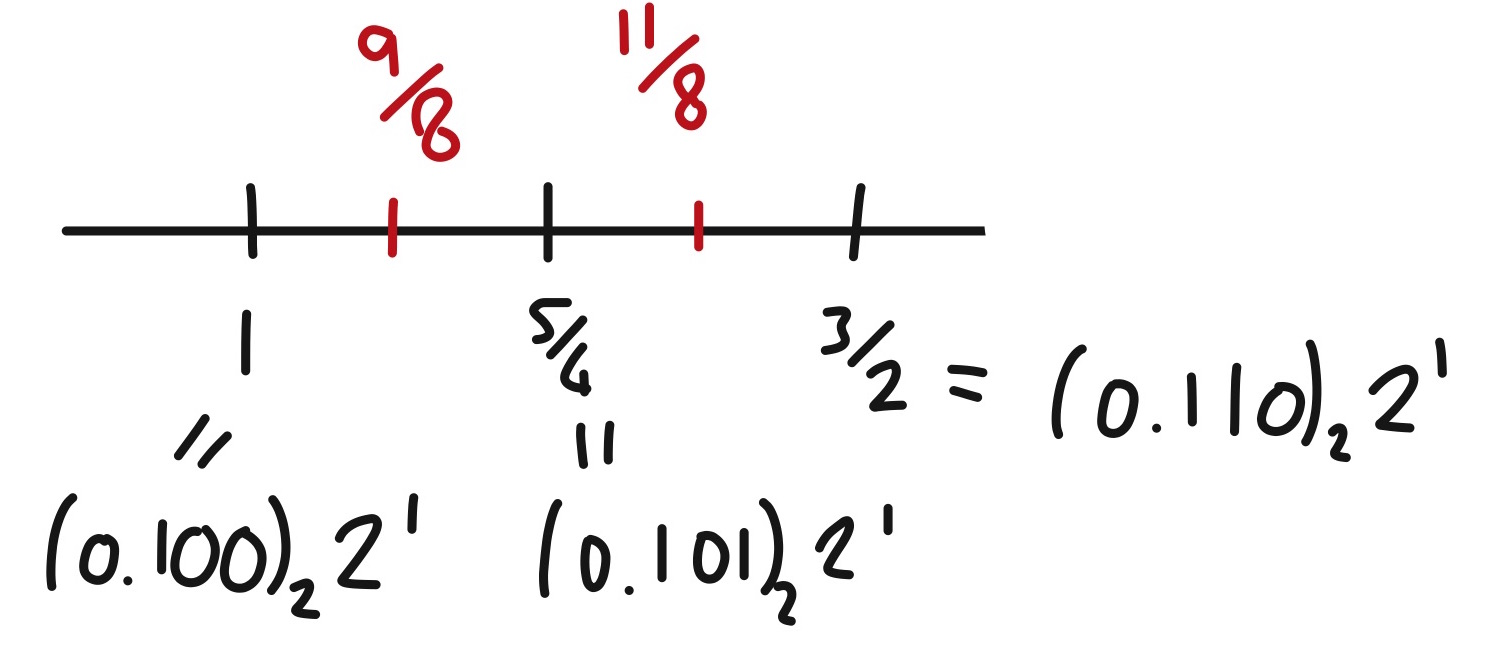
\includegraphics[width=0.7\linewidth,height=\textheight,keepaspectratio]{im/fp2.jpg}
\end{center}

\(\tfrac98 = (1.001)_2\) has neighbours \(1 = (0.100)_22^1\) and
\(\tfrac54 = (0.101)_22^1\), so is rounded down to \(1\).\\
\(\tfrac{11}{8} = (1.011)_2\) has neighbours \(\tfrac54 = (0.101)_22^1\)
and \(\tfrac32=(0.110)_22^1\), so is rounded up to \(\tfrac32\).

\begin{tcolorbox}[enhanced jigsaw, bottomtitle=1mm, title=\textcolor{quarto-callout-note-color}{\faInfo}\hspace{0.5em}{Note}, colback=white, opacityback=0, rightrule=.15mm, bottomrule=.15mm, colbacktitle=quarto-callout-note-color!10!white, colframe=quarto-callout-note-color-frame, arc=.35mm, breakable, coltitle=black, leftrule=.75mm, left=2mm, toptitle=1mm, toprule=.15mm, titlerule=0mm, opacitybacktitle=0.6]

\textbf{Vancouver stock exchange index:} In 1982, the index was
established at 1000. By November 1983, it had fallen to 520, even though
the exchange seemed to be doing well. Explanation: the index was rounded
\emph{down} to 3 digits at every recomputation. Since the errors were
always in the same direction, they added up to a large error over time.
Upon recalculation, the index doubled!

\end{tcolorbox}

\section{Significant figures}\label{significant-figures}

When doing calculations without a computer, we often use the terminology
of \textbf{significant figures}. To count the number of significant
figures in a number \(x\), start with the first non-zero digit from the
left, and count all the digits thereafter, including final zeros if they
are after the decimal point.

To round \(x\) to \(n\) s.f., replace \(x\) by the nearest number with
\(n\) s.f. An approximation \(\hat{x}\) of \(x\) is ``correct to \(n\)
s.f.'' if both \(\hat{x}\) and \(x\) round to the same number to \(n\)
s.f.

\section{Rounding error}\label{rounding-error}

If \(|x|\) lies between the smallest non-zero number in \(F\) and the
largest number in \(F\), then \[
\mathrm{fl}(x) = x(1+\delta),
\] where the relative error incurred by rounding is \[
|\delta| = \frac{|\mathrm{fl}(x) - x|}{|x|}.
\]

\begin{tcolorbox}[enhanced jigsaw, bottomtitle=1mm, title=\textcolor{quarto-callout-note-color}{\faInfo}\hspace{0.5em}{Note}, colback=white, opacityback=0, rightrule=.15mm, bottomrule=.15mm, colbacktitle=quarto-callout-note-color!10!white, colframe=quarto-callout-note-color-frame, arc=.35mm, breakable, coltitle=black, leftrule=.75mm, left=2mm, toptitle=1mm, toprule=.15mm, titlerule=0mm, opacitybacktitle=0.6]

Relative errors are often more useful because they are scale invariant.
E.g., an error of 1 hour is irrelevant in estimating the age of this
lecture theatre, but catastrophic in timing your arrival at the lecture.

\end{tcolorbox}

Now \(x\) may be written as \(x=(0.d_1d_2\cdots)_\beta\beta^e\) for some
\(e\in[e_{\rm min},e_{\rm max}]\), but the fraction will not terminate
after \(m\) digits if \(x\notin F\). However, this fraction will differ
from that of \(\mathrm{fl}(x)\) by at most \(\tfrac12\beta^{-m}\), so \[
|\mathrm{fl}(x) - x| \leq \tfrac12\beta^{-m}\beta^e \quad \implies \quad |\delta| \leq \tfrac12\beta^{1-m}.
\] Here we used that the fractional part of \(|x|\) is at least
\((0.1)_\beta \equiv \beta^{-1}\). The number
\(\epsilon_{\rm M} = \tfrac12\beta^{1-m}\) is called the \textbf{machine
epsilon} (or \textbf{unit roundoff}), and is independent of \(x\). So
the relative rounding error satisfies \[
|\delta| \leq \epsilon_{\rm M}.
\]

\begin{tcolorbox}[enhanced jigsaw, bottomtitle=1mm, title=\textcolor{quarto-callout-note-color}{\faInfo}\hspace{0.5em}{Note}, colback=white, opacityback=0, rightrule=.15mm, bottomrule=.15mm, colbacktitle=quarto-callout-note-color!10!white, colframe=quarto-callout-note-color-frame, arc=.35mm, breakable, coltitle=black, leftrule=.75mm, left=2mm, toptitle=1mm, toprule=.15mm, titlerule=0mm, opacitybacktitle=0.6]

To check the machine epsilon value in Matlab you can just type `eps' in
the command line, which will return the value 2.2204e-16.

\end{tcolorbox}

\begin{tcolorbox}[enhanced jigsaw, bottomtitle=1mm, title=\textcolor{quarto-callout-note-color}{\faInfo}\hspace{0.5em}{Note}, colback=white, opacityback=0, rightrule=.15mm, bottomrule=.15mm, colbacktitle=quarto-callout-note-color!10!white, colframe=quarto-callout-note-color-frame, arc=.35mm, breakable, coltitle=black, leftrule=.75mm, left=2mm, toptitle=1mm, toprule=.15mm, titlerule=0mm, opacitybacktitle=0.6]

The name ``unit roundoff'' arises because \(\beta^{1-m}\) is the
distance between 1 and the next number in the system.

\end{tcolorbox}

When adding/subtracting/multiplying/dividing two numbers in \(F\), the
result will not be in \(F\) in general, so must be rounded.

Let us multiply \(x=\tfrac58\) and \(y=\tfrac78\). We have \[
xy = \tfrac{35}{64} = \tfrac12 + \tfrac1{32} + \tfrac1{64} = (0.100011)_2.
\] This has too many significant digits to represent in our system, so
the best we can do is round the result to
\(\mathrm{fl}(xy) = (0.100)_2 = \tfrac12\).

\begin{tcolorbox}[enhanced jigsaw, bottomtitle=1mm, title=\textcolor{quarto-callout-note-color}{\faInfo}\hspace{0.5em}{Note}, colback=white, opacityback=0, rightrule=.15mm, bottomrule=.15mm, colbacktitle=quarto-callout-note-color!10!white, colframe=quarto-callout-note-color-frame, arc=.35mm, breakable, coltitle=black, leftrule=.75mm, left=2mm, toptitle=1mm, toprule=.15mm, titlerule=0mm, opacitybacktitle=0.6]

Typically additional digits are used during the computation itself, as
in our example.

\end{tcolorbox}

For \({\circ} = +,-,\times, \div\), IEEE standard arithmetic requires
rounded exact operations, so that \[
\mathrm{fl}(x {\,\circ\,} y) = (x {\,\circ\,} y)(1+\delta), \quad |\delta|\leq\epsilon_{\rm M}.
\]

\section{Loss of significance}\label{loss-of-significance}

You might think that the above guarantees the accuracy of calculations
to within \(\epsilon_{\rm M}\), but this is true only if \(x\) and \(y\)
are themselves exact. In reality, we are probably starting from
\(\bar{x}=x(1+\delta_1)\) and \(\bar{y}=y(1 + \delta_2)\), with
\(|\delta_1|, |\delta_2| \leq \epsilon_{\rm M}\). In that case, there is
an error even before we round the result, since \[
\begin{aligned}
\bar{x} \pm \bar{y} &= x(1+ \delta_1) \pm y(1 + \delta_2)\\
&= (x\pm y)\left(1 + \frac{x\delta_1 \pm y\delta_2}{x\pm y}\right).
\end{aligned}
\] If the correct answer \(x\pm y\) is very small, then there can be an
arbitrarily large relative error in the result, compared to the errors
in the initial \(\bar{x}\) and \(\bar{y}\). In particular, this relative
error can be much larger than \(\epsilon_{\rm M}\). This is called
\textbf{loss of significance}, and is a major cause of errors in
floating-point calculations.

To 4 s.f., the roots are \[
x_1 = 28 + \sqrt{783} = 55.98, \quad x_2 = 28-\sqrt{783} = 0.01786.
\] However, working to 4 s.f. we would compute \(\sqrt{783} = 27.98\),
which would lead to the results \[
\bar{x}_1 = 55.98, \quad \bar{x}_2 = 0.02000.
\] The smaller root is not correct to 4 s.f., because of cancellation
error. One way around this is to note that
\(x^2 - 56x + 1 = (x-x_1)(x-x_2)\), and compute \(x_2\) from
\(x_2 = 1/x_1\), which gives the correct answer.

\begin{tcolorbox}[enhanced jigsaw, bottomtitle=1mm, title=\textcolor{quarto-callout-note-color}{\faInfo}\hspace{0.5em}{Note}, colback=white, opacityback=0, rightrule=.15mm, bottomrule=.15mm, colbacktitle=quarto-callout-note-color!10!white, colframe=quarto-callout-note-color-frame, arc=.35mm, breakable, coltitle=black, leftrule=.75mm, left=2mm, toptitle=1mm, toprule=.15mm, titlerule=0mm, opacitybacktitle=0.6]

Note that the error crept in when we rounded \(\sqrt{783}\) to
\(27.98\), because this removed digits that would otherwise have been
significant after the subtraction.

\end{tcolorbox}

Let us plot this function in the range
\(-5\times 10^{-8}\leq x \leq 5\times 10^{-8}\) -- even in IEEE double
precision arithmetic we find significant errors, as shown by the blue
curve:

\begin{center}
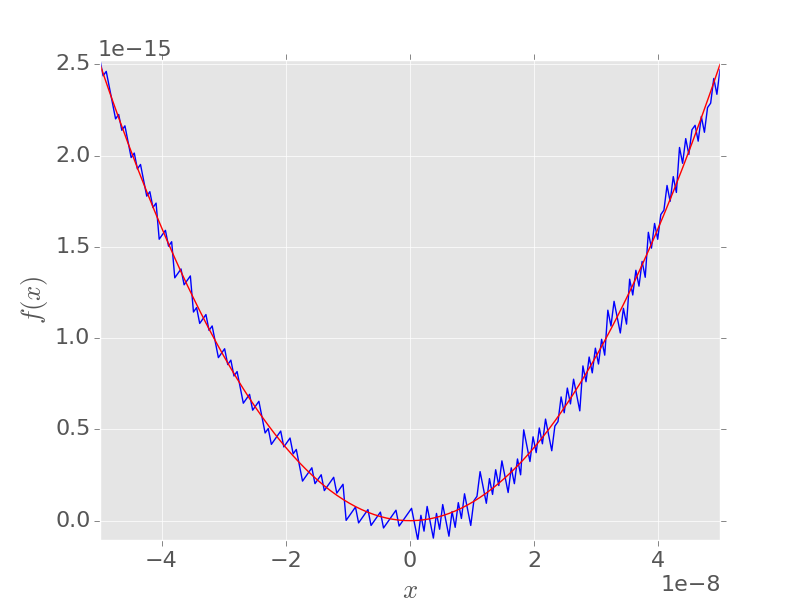
\includegraphics[width=0.7\linewidth,height=\textheight,keepaspectratio]{im/floating1.png}
\end{center}

The red curve shows the correct result approximated using the Taylor
series \[
\begin{aligned}
f(x) &= \left(1 + x + \frac{x^2}{2!} + \frac{x^3}{3!} + \ldots\right) - \left( 1 - \frac{x^2}{2!} + \frac{x^4}{4!} - \ldots\right) - x\\
&\approx x^2 + \frac{x^3}{6}.
\end{aligned}
\] This avoids subtraction of nearly equal numbers.

\begin{tcolorbox}[enhanced jigsaw, bottomtitle=1mm, title=\textcolor{quarto-callout-note-color}{\faInfo}\hspace{0.5em}{Note}, colback=white, opacityback=0, rightrule=.15mm, bottomrule=.15mm, colbacktitle=quarto-callout-note-color!10!white, colframe=quarto-callout-note-color-frame, arc=.35mm, breakable, coltitle=black, leftrule=.75mm, left=2mm, toptitle=1mm, toprule=.15mm, titlerule=0mm, opacitybacktitle=0.6]

We will look in more detail at polynomial approximations in the next
section.

\end{tcolorbox}

Note that floating-point arithmetic violates many of the usual rules of
real arithmetic, such as \((a+b)+c = a + (b+c)\).

\[
\begin{aligned}
\mathrm{fl}\big[(5.9 + 5.5) + 0.4\big] &= \mathrm{fl}\big[\mathrm{fl}(11.4) + 0.4\big] = \mathrm{fl}(11.0 + 0.4) = 11.0,\\
\mathrm{fl}\big[5.9 + (5.5 + 0.4)\big] &= \mathrm{fl}\big[5.9 + 5.9 \big] = \mathrm{fl}(11.8) = 12.0.
\end{aligned}
\]

In \(\mathbb{R}\), the average of two numbers always lies between the
numbers. But if we work to 3 decimal digits, \[
\mathrm{fl}\left(\frac{5.01 + 5.02}{2}\right) = \frac{\mathrm{fl}(10.03)}{2} = \frac{10.0}{2} = 5.0.
\]

The moral of the story is that sometimes care is needed to ensure that
we carry out a calculation accurately and as intended!

\section*{Knowledge checklist}\label{knowledge-checklist}
\addcontentsline{toc}{section}{Knowledge checklist}

\markright{Knowledge checklist}

\textbf{Key topics:}

\begin{enumerate}
\def\labelenumi{\arabic{enumi}.}
\item
  Integer and floating point representations of real numbers on
  computers.
\item
  Overflow, underflow and loss of significance.
\end{enumerate}

\textbf{Key skills:}

\begin{itemize}
\item
  Understanding and distinguishing integer, fixed-point, and
  floating-point representations.
\item
  Analyzing the effects of rounding and machine epsilon in calculations.
\item
  Diagnosing and managing rounding errors, overflow, and underflow.
\end{itemize}

\bookmarksetup{startatroot}

\chapter{Continuous Functions}\label{continuous-functions}

The goal of this chapter is to explore and begin to answer the following
question:

\begin{quote}
\emph{How do we represent mathematical functions on a computer?}
\end{quote}

\section*{Polynomial Interpolation:
Motivation}\label{polynomial-interpolation-motivation}
\addcontentsline{toc}{section}{Polynomial Interpolation: Motivation}

\markright{Polynomial Interpolation: Motivation}

If \(f\) is a polynomial of degree \(n\), \[
f(x) = p_n(x) = a_0 + a_1x + \ldots + a_nx^n,
\] then we only need to store the \(n+1\) coefficients
\(a_0,\ldots,a_n\). Operations such as taking the derivative or
integrating \(f\) are also convenient. The idea in this chapter is to
find a polynomial that approximates a general function \(f\). For a
continuous function \(f\) on a bounded interval, this is always possible
if you take a high enough degree polynomial:

\phantomsection\label{WAT}
\begin{fbxSimple}{theorem}{Theorem 2.1: }{Weierstrass Approximation Theorem (1885)}
\phantomsection\label{WAT}
For any \(f\in C([0,1])\) and any \(\epsilon > 0\), there exists a
polynomial \(p(x)\) such that \[
\max_{0\leq x\leq 1}\big|f(x) - p(x)\big| \leq \epsilon.
\]

\end{fbxSimple}

\begin{tcolorbox}[enhanced jigsaw, bottomtitle=1mm, title=\textcolor{quarto-callout-note-color}{\faInfo}\hspace{0.5em}{Note}, colback=white, opacityback=0, rightrule=.15mm, bottomrule=.15mm, colbacktitle=quarto-callout-note-color!10!white, colframe=quarto-callout-note-color-frame, arc=.35mm, breakable, coltitle=black, leftrule=.75mm, left=2mm, toptitle=1mm, toprule=.15mm, titlerule=0mm, opacitybacktitle=0.6]

This may be proved using an explicit sequence of polynomials, called
Bernstein polynomials.

\end{tcolorbox}

If \(f\) is not continuous, then something other than a polynomial is
required, since polynomials can't handle asymptotic behaviour.

\begin{tcolorbox}[enhanced jigsaw, bottomtitle=1mm, title=\textcolor{quarto-callout-note-color}{\faInfo}\hspace{0.5em}{Note}, colback=white, opacityback=0, rightrule=.15mm, bottomrule=.15mm, colbacktitle=quarto-callout-note-color!10!white, colframe=quarto-callout-note-color-frame, arc=.35mm, breakable, coltitle=black, leftrule=.75mm, left=2mm, toptitle=1mm, toprule=.15mm, titlerule=0mm, opacitybacktitle=0.6]

To approximate functions like \(1/x\), there is a well-developed theory
of rational function interpolation, which is beyond the scope of this
course.

\end{tcolorbox}

In this chapter, we look for a suitable polynomial \(p_n\) by
\textbf{interpolation}---that is, requiring \(p_n(x_i) = f(x_i)\) at a
finite set of points \(x_i\), usually called \textbf{nodes}. Sometimes
we will also require the derivative(s) of \(p_n\) to match those of
\(f\).

\section*{Taylor series}\label{taylor-series}
\addcontentsline{toc}{section}{Taylor series}

\markright{Taylor series}

A truncated Taylor series is (in some sense) the simplest interpolating
polynomial since it uses only a single node \(x_0\), although it does
require \(p_n\) to match both \(f\) and some of its derivatives.

We can approximate this using a Taylor series about the point \(x_0=0\),
which is \[
\sin(x) = x - \frac{x^3}{3!} + \frac{x^5}{5!} - \frac{x^7}{7!} + \ldots.
\] This comes from writing \[
f(x) = a_0 + a_1(x-x_0) + a_2(x-x_0)^2 + \ldots,
\] then differentiating term-by-term and matching values at \(x_0\):
\begin{align*}
f(x_0) &= a_0,\\
f'(x_0) &= a_1,\\
f''(x_0) &= 2a_2,\\
f'''(x_0) &= 3(2)a_3,\\
&\vdots\\
\implies f(x) &= f(x_0) + f'(x_0)(x-x_0) + \frac{f''(x_0)}{2!}(x-x_0)^2 + \frac{f'''(x_0)}{3!}(x-x_0)^3 + \ldots.
\end{align*} So \begin{align*}
\textrm{1 term} \;&\implies\; f(0.1) \approx 0.1,\\
\textrm{2 terms} \;&\implies\; f(0.1) \approx 0.1 - \frac{0.1^3}{6} = 0.099833\ldots,\\
\textrm{3 terms} \;&\implies\; f(0.1) \approx 0.1 - \frac{0.1^3}{6} + \frac{0.1^5}{120} = 0.09983341\ldots.\\
\end{align*} The next term will be
\(-0.1^7/7! \approx -10^{-7}/10^3 = -10^{-10}\), which won't change the
answer to 6 s.f.

\begin{tcolorbox}[enhanced jigsaw, bottomtitle=1mm, title=\textcolor{quarto-callout-note-color}{\faInfo}\hspace{0.5em}{Note}, colback=white, opacityback=0, rightrule=.15mm, bottomrule=.15mm, colbacktitle=quarto-callout-note-color!10!white, colframe=quarto-callout-note-color-frame, arc=.35mm, breakable, coltitle=black, leftrule=.75mm, left=2mm, toptitle=1mm, toprule=.15mm, titlerule=0mm, opacitybacktitle=0.6]

The exact answer is \(\sin(0.1)=0.09983341\).

\end{tcolorbox}

Mathematically, we can write the remainder as follows.

\phantomsection\label{taylors-theorem}
\begin{fbxSimple}{theorem}{Theorem 2.2: }{Taylor’s Theorem}
\phantomsection\label{taylors-theorem}
Let \(f\) be \(n+1\) times differentiable on \((a,b)\), and let
\(f^{(n)}\) be continuous on \([a,b]\). If \(x,x_0\in[a,b]\) then there
exists \(\xi \in (a,b)\) such that \[
f(x) = \sum_{k=0}^n\frac{f^{(k)}(x_0)}{k!}(x-x_0)^k \; + \; \frac{f^{(n+1)}(\xi)}{(n+1)!}(x-x_0)^{n+1}.
\]

\end{fbxSimple}

The sum is called the \textbf{Taylor polynomial} of degree \(n\), and
the last term is called the \textbf{Lagrange form} of the remainder.
Note that the unknown number \(\xi\) depends on \(x\).

For \(f(x)=\sin(x)\), we found the Taylor polynomial
\(p_6(x) = x - x^3/3! + x^5/5!\), and \(f^{(7)}(x)=-\sin(x)\). So we
have \[
\big|f(x) - p_6(x)\big| = \left|\frac{f^{(7)}(\xi)}{7!}(x-x_0)^7\right|
\] for some \(\xi\) between \(x_0\) and \(x\). For \(x=0.1\), we have \[
\big|f(0.1) - p_6(0.1)\big| = \frac{1}{5040}(0.1)^7\big|f^{(7)}(\xi)\big| \quad \textrm{for some $\xi\in[0,0.1]$}.
\] Since \(\big|f^{(7)}(\xi)\big| = \big|\sin(\xi)\big| \leq 1\), we can
say, before calculating, that the error satisfies \[
\big|f(0.1) - p_6(0.1)\big| \leq 1.984\times 10^{-11}.
\]

\begin{tcolorbox}[enhanced jigsaw, bottomtitle=1mm, title=\textcolor{quarto-callout-note-color}{\faInfo}\hspace{0.5em}{Note}, colback=white, opacityback=0, rightrule=.15mm, bottomrule=.15mm, colbacktitle=quarto-callout-note-color!10!white, colframe=quarto-callout-note-color-frame, arc=.35mm, breakable, coltitle=black, leftrule=.75mm, left=2mm, toptitle=1mm, toprule=.15mm, titlerule=0mm, opacitybacktitle=0.6]

The actual error is \(1.983\times 10^{-11}\), so this is a tight
estimate.

\end{tcolorbox}

Since this error arises from approximating \(f\) with a truncated
series, rather than due to rounding, it is known as \textbf{truncation
error}. Note that it tends to be lower if you use more terms (larger
\(n\)), or if the function oscillates less (smaller \(f^{(n+1)}\) on the
interval \((x_0,x)\)).

Error estimates like the Lagrange remainder play an important role in
numerical analysis and computation, so it is important to understand
where it comes from. The number \(\xi\) will ultimately come from
Rolle's theorem, which is a special case of the mean value theorem from
first-year calculus:

\phantomsection\label{rolles-theorem}
\begin{fbxSimple}{theorem}{Theorem 2.3: }{Rolle’s Theorem}
\phantomsection\label{rolles-theorem}
If \(f\) is continuous on \([a,b]\) and differentiable on \((a,b)\),
with \(f(a)=f(b)=0\), then there exists \(\xi\in(a,b)\) with
\(f'(\xi)=0\).

\end{fbxSimple}

\textbf{Proof of Lagrange remainder (Taylor's Theorem)}

The argument goes as follows:

\begin{enumerate}
\def\labelenumi{\arabic{enumi}.}
\tightlist
\item
  Define the ``auxiliary'' function\\
  \[
  g(t) = f(t) - p_n(t) - M(t-x_0)^{n+1},
  \] where \(p_n\) is the Taylor polynomial. By construction, this
  function satisfies \[
  \begin{aligned}
  g(x_0) &= f(x_0) - p_n(x_0) - M(0)^{n+1} = 0,\\
  g'(x_0) &= f'(x_0) - p_n'(x_0) - (n+1)M(0)^{n} = 0,\\
  g''(x_0) &= f''(x_0) - p_n''(x_0) - n(n+1)M(0)^{n-1} = 0,\\
  &\vdots\\
  g^{(n)}(x_0) &= f^{(n)}(x_0) - p_n^{(n)}(x_0) - (n+1)!M(0) = 0.
  \end{aligned}
  \]
\item
  By a suitable choice of \(M\), we can make \(g(x)=0\) too. Put\\
  \[
  M = \frac{f(x) - p_n(x)}{(x-x_0)^{n+1}},
  \] then \(g(x) = f(x) - p_n(x) - M(x-x_0)^{n+1} = 0\).
\item
  Since \(g(x_0)=g(x)=0\) and \(x\neq x_0\), Rolle's theorem implies
  that there exists \(\xi_0\) between \(x_0\) and \(x\) such that
  \(g'(\xi_0)=0\). But we already know that \(g'(x_0)=0\), so \(g'\) has
  two distinct roots and we can apply Rolle's theorem again. Hence there
  exists \(\xi_1\) between \(x_0\) and \(\xi_0\) such that
  \(g''(\xi_1)=0\). We can keep repeating this argument until we get
  \(\xi_{n+1}\equiv \xi\) such that \(g^{(n+1)}(\xi)=0\).
\item
  We can differentiate \(g(t)\) to see that\\
  \[
  g^{(n+1)}(t) = f^{(n+1)}(t) - p_n^{(n+1)}(t) - M \frac{\mathrm{d}^{n+1}}{\mathrm{d}t^{n+1}}\big[(t-x_0)^{n+1}\big] = f^{(n+1)}(t) - M(n+1)!
  \] Substituting \(\xi\) and our chosen \(M\) gives\\
  \[
  0 = g^{(n+1)}(\xi) = f^{(n+1)}(\xi) - \frac{f(x) - p_n(x)}{(x-x_0)^{n+1}}(n+1)!
  \] which rearranges to give the formula in Taylor's Theorem.
\end{enumerate}

\section{Polynomial interpolation}\label{polynomial-interpolation}

The classical problem of \textbf{polynomial interpolation} is to find a
polynomial \[
p_n(x) = a_0 + a_1x + \ldots + a_n x^n = \sum_{k=0}^n a_k x^k
\] that interpolates our function \(f\) at a finite set of nodes
\(\{x_0, x_1, \ldots, x_m\}\). In other words, \(p_n(x_i)=f(x_i)\) at
each of the nodes \(x_i\). Since the polynomial has \(n+1\) unknown
coefficients, we expect to need \(n+1\) distinct nodes, so let us assume
that \(m=n\).

Here we have two nodes \(x_0\), \(x_1\), and seek a polynomial
\(p_1(x) = a_0 + a_1x\). Then the interpolation conditions require that
\[
\begin{cases}
p_1(x_0) = a_0 + a_1x_0 = f(x_0)\\
p_1(x_1) = a_0 + a_1x_1 = f(x_1)
\end{cases}
\implies\quad
p_1(x) = \frac{x_1f(x_0) - x_0f(x_1)}{x_1 - x_0} + \frac{f(x_1) - f(x_0)}{x_1 - x_0}x.
\]

For general \(n\), the interpolation conditions require \[
\begin{matrix}
a_0 &+& a_1x_0 &+& a_2x_0^2 &+& \ldots &+& a_nx_0^n &=& f(x_0),\\
a_0 &+& a_1x_1 &+& a_2x_1^2 &+& \ldots &+& a_nx_1^n &=& f(x_1),\\
\vdots  && \vdots  && \vdots     &&        &&\vdots      && \vdots\\
a_0 &+& a_1x_n &+& a_2x_n^2 &+& \ldots &+& a_nx_n^n &=& f(x_n),
\end{matrix}
\] so we have to solve \[
\begin{pmatrix}
1 & x_0 & x_0^2 & \cdots & x_0^n\\
1 & x_1 & x_1^2 & \cdots & x_1^n\\
\vdots & \vdots &\vdots& & \vdots\\
1 & x_n & x_n^2 & \cdots & x_n^n\\
\end{pmatrix}
\begin{pmatrix}
a_0\\ a_1\\ \vdots\\ a_n
\end{pmatrix}
=
\begin{pmatrix}
f(x_0)\\ f(x_1)\\ \vdots\\ f(x_n)
\end{pmatrix}.
\] This is called a \textbf{Vandermonde matrix}. The determinant of this
matrix is \[
\det(A) = \prod_{0\leq i < j\leq n} (x_j - x_i),
\] which is non-zero provided the nodes are all distinct. This
establishes an important result, where \(\mathcal{P}_n\) denotes the
space of all real polynomials of degree \(\leq n\).

\phantomsection\label{existenceuniqueness}
\begin{fbxSimple}{theorem}{Theorem 2.4: }{Existence/uniqueness}
\phantomsection\label{existenceuniqueness}
Given \(n+1\) distinct nodes \(x_0, x_1, \ldots, x_n\), there is a
unique polynomial \(p_n\in\mathcal{P}_n\) that interpolates \(f(x)\) at
these nodes.

\end{fbxSimple}

We may also prove uniqueness by the following elegant argument.

\textbf{Proof (Uniqueness part of Existence/Uniqueness Theorem):}\\
Suppose that in addition to \(p_n\) there is another interpolating
polynomial \(q_n\in\mathcal{P}_n\). Then the difference
\(r_n := p_n - q_n\) is also a polynomial with degree \(\leq n\). But we
have \[
r_n(x_i) = p_n(x_i) - q_n(x_i) = f(x_i)-f(x_i)=0 \quad \textrm{for $i=0,\ldots,n$},
\] so \(r_n(x)\) has \(n+1\) roots. From the Fundamental Theorem of
Algebra, this is possible only if \(r_n(x)\equiv 0\), which implies that
\(q_n=p_n\).

\begin{tcolorbox}[enhanced jigsaw, bottomtitle=1mm, title=\textcolor{quarto-callout-note-color}{\faInfo}\hspace{0.5em}{Note}, colback=white, opacityback=0, rightrule=.15mm, bottomrule=.15mm, colbacktitle=quarto-callout-note-color!10!white, colframe=quarto-callout-note-color-frame, arc=.35mm, breakable, coltitle=black, leftrule=.75mm, left=2mm, toptitle=1mm, toprule=.15mm, titlerule=0mm, opacitybacktitle=0.6]

Note that the unique polynomial through \(n+1\) points may have degree
\(< n\). This happens when \(a_0=0\) in the solution to the Vandermonde
system above.

\end{tcolorbox}

We have \(x_0=0\), \(x_1=\tfrac{\pi}{2}\), \(x_2=\pi\), so \(f(x_0)=1\),
\(f(x_1)=0\), \(f(x_2)=-1\). Clearly the unique interpolant is a
straight line \(p_2(x) = 1 - \tfrac2\pi x\).

If we took the nodes \(\{0,2\pi,4\pi\}\), we would get a constant
function \(p_2(x)=1\).

\begin{center}
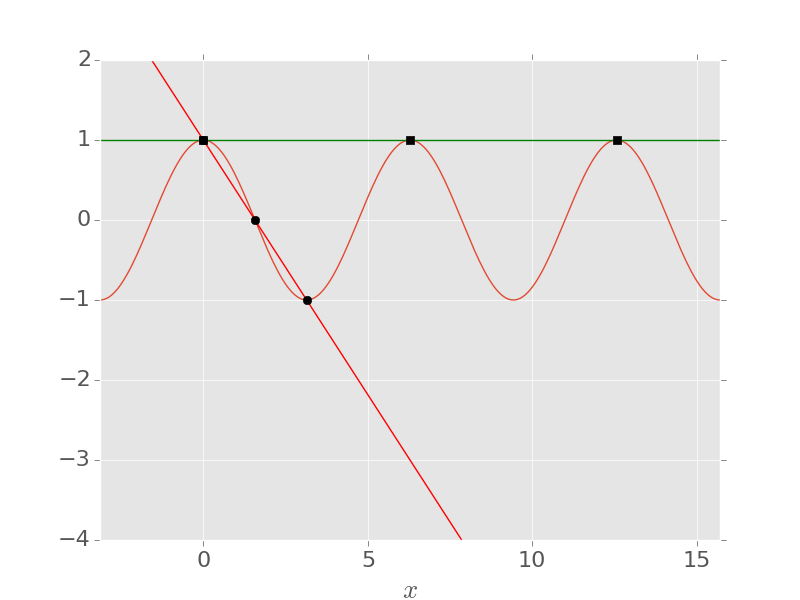
\includegraphics[width=0.7\linewidth,height=\textheight,keepaspectratio]{im/linear_interp.png}
\end{center}

One way to compute the interpolating polynomial would be to solve the
Vandermonde system above, e.g.~by Gaussian elimination. However, we will
see (next term) that this is not recommended. In practice, we choose a
different basis for \(p_n\). There are two common choices, due to
Lagrange and Newton.

\begin{tcolorbox}[enhanced jigsaw, bottomtitle=1mm, title=\textcolor{quarto-callout-note-color}{\faInfo}\hspace{0.5em}{Note}, colback=white, opacityback=0, rightrule=.15mm, bottomrule=.15mm, colbacktitle=quarto-callout-note-color!10!white, colframe=quarto-callout-note-color-frame, arc=.35mm, breakable, coltitle=black, leftrule=.75mm, left=2mm, toptitle=1mm, toprule=.15mm, titlerule=0mm, opacitybacktitle=0.6]

The Vandermonde matrix arises when we write \(p_n\) in the
\textbf{natural basis} \(\{1,x,x^2,\ldots\}\).

\end{tcolorbox}




\end{document}
